\documentclass[a4paper]{article}
\usepackage{graphicx}
\usepackage{xcolor}
\usepackage{titlesec, titletoc} %设置标题格式
\usepackage{xeCJK}
\usepackage{fontspec} 
\usepackage{geometry}
\usepackage{fancyhdr}
\usepackage{mdframed}
\usepackage{listings}
\usepackage{amsmath,amssymb}
\usepackage{multirow}
\usepackage{float}
\usepackage{booktabs}
\usepackage{url}
\usepackage{hyperref}
\usepackage{array}
\usepackage[toc,page,title,titletoc,header]{appendix} 
\usepackage{enumerate}
\usepackage{subfig}
\usepackage{natbib}

% \renewcommand{\thefigure}{\thesection-\arabic{figure}}

\linespread{1.3}

\definecolor{codegreen}{rgb}{0,0.6,0}
\definecolor{codegray}{rgb}{0.5,0.5,0.5}
\definecolor{codepurple}{rgb}{0.58,0,0.82}
\definecolor{backcolour}{rgb}{0.95,0.95,0.92}
\definecolor{codeblack}{rgb}{255,255,255}

\lstdefinestyle{mystyle}{
	backgroundcolor=\color{backcolour},   
	commentstyle=\color{codegreen},
	% keywordstyle=\color{magenta},
	keywordstyle=\color{blue!70},
	numberstyle=\tiny\color{codegray},
	stringstyle=\color{codepurple},
	basicstyle=\footnotesize,
	breakatwhitespace=false,         
	breaklines=true,                 
	captionpos=b,                    
	keepspaces=true,                 
	numbers=left,                    
	numbersep=5pt,                  
	showspaces=false,                
	showstringspaces=false,
	showtabs=false,                  
	tabsize=4,
}
\lstset{style=mystyle}

\geometry{left=2.5cm,right=2.5cm,top=2.5cm,bottom=2.5cm}

% \renewcommand{\thefootnote}{\fnsymbol{footnote}}

\pagestyle{fancy}
\definecolor{dhscodebg}{rgb}{0.85,0.85,0.85}
\newcommand{\HUGE}{\fontsize{29pt}{29pt}\selectfont}

\setmainfont[Mapping=tex-text]{STSONG.TTF}
\lhead{Matlab高级编程与工程应用}
\chead{图像处理大作业实验报告}
\rhead{王禹\ 2014011241 }
\cfoot{\thepage}
\begin{document}
	\pagenumbering{gobble}	
	\begin{titlepage}
		\phantom{Start!}
		\vspace{5cm}
		\begin{center}
			{ \HUGE \bfseries  Matlab高级编程与工程应用}\\[0.4cm]
			{ \HUGE \bfseries  图像处理大作业实验报告}\\[0.4cm]
		\end{center}
		\begin{flushright}
			\vfill
			{
				\newcommand{\pillar}{ {\Huge \phantom{A}} }
				\large
				\begin{tabular}{lc}
					\pillar 姓名 & 王禹 \\
					\pillar 学号 & 2014011241\\
					\pillar 班级 & 无48\\
					\pillar 日期 & 二〇一六年\ 八月\ 二十五日 \\
				\end{tabular}
			}
		\end{flushright}
	\end{titlepage}
	\renewcommand{\contentsname}{目录}
	\tableofcontents
	\newpage
	\pagenumbering{arabic}
	\section{原创性声明}
	本实验完全采用原创设计代码,仅在自主设计JPEG信息隐藏的时候,参考了李思涵同学的思想。
	\section{实验目的}
	\begin{itemize}
		\item 了解计算机存储和处理图像的基础知识;
		\item 掌握JPEG标准的基本原理;
		\item 变化域编码和量化的基本思想;
		\item MATLAB处理矩阵和图像的常用命令;
		\item 在变换域进行信息隐藏的方法;
		\item 学习人脸检测的基本方法。
	\end{itemize}
	
	\section{基础知识}
	\subsection{MATLAB提供了图像处理工具箱,请阅读并大致了解这些函数的基本功能}
	\subsection{利用MATLAB提供的Image file I/O函数分别完成以下处理:}
	\subsubsection{以测试图像的中心为圆心,图像的长和宽中较小值的一半为半径画一个红色的圆;}
	
	图像的读写IO主要依靠MATLAB自带的图像处理工具箱的imread和imwrite函数。将图像读入后,彩色图像为三维矩阵,灰度矩阵为二维矩阵。而本实验中,则是直接load已经准备好的.mat文件,获得图像矩阵。彩色图像的前两维分别为高和宽的像素值,第三维按照顺序为RGB,矩阵的值为0~255的RGB三色的亮度值;灰度图像则没有第三维,只有一个灰度亮度值的二维矩阵。第一问直接获得了图像的矩阵后,找到距离中心小于所指定半径的所有点,将其R分量值调为255,G和B分量都调为0,即可得到所需的图像,最终的结果如下图Figure~\ref{fig1:fi1}所示,而代码如Listing~\ref{lst1:lst1}所示。
	
	\begin{figure}[b]
			\centering
			\subfloat[红圆\label{fig1:fi1}]{
				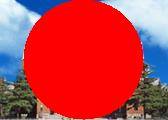
\includegraphics[width = .35\textwidth]{../source/3.1/a.jpg}
			}
			\hspace{0.75cm}
			\subfloat[棋格\label{fig1:fi2}]{
				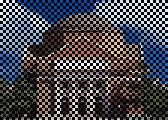
\includegraphics[width = .35\textwidth]{../source/3.1/b.jpg}
			}	
			\caption{题3.1~结果图}
			\label{fig1}
	\end{figure}
	

	\subsubsection{将测试图像涂成国际象棋状的“黑白格”的样子,其中“黑”即为黑色,“白”则意味着保留原图。}
	对于分割为棋盘,为了判断是涂黑还是保持原样,只需判断所要处理的格子的横纵坐标序列数之和的奇偶性即可。结果图见Figure~\ref{fig1:fi2},具体代码见Listing~\ref{lst1:lst2}。
	
	\lstinputlisting[language=Matlab,caption=画红色圆代码,label=lst1:lst1,frame=shadowbox,
	backgroundcolor=\color{white}, rulesepcolor=\color{red!10!green!10!blue!10},,xleftmargin=2em,xrightmargin=2em, aboveskip=1em]{../source/3.1/a.m} 
	
	\lstinputlisting[language=Matlab,caption=涂棋格代码,label=lst1:lst2,frame=shadowbox,
	backgroundcolor=\color{white}, rulesepcolor=\color{red!10!green!10!blue!10},,xleftmargin=2em,xrightmargin=2em, aboveskip=1em]{../source/3.1/b.m} 	
	
	
	\section{图像压缩编码}
	\subsection{图像的预处理是将每个像素灰度值减去128,这个步骤是否可以在变换域进行?} 
	由于变换域的第一个分量便是直流分量,因此这个步骤可以在变换域进行。块是$8 \times 8$ 的像素块,他的DC分量基底为$\frac{1}{8}$,因此将DCT变换后的直流分量减去128即可得到预处理图像。具体代码见Listing~\ref{lst2:lst1}。
	
	根据结果来看,结果相差为$10^{-13}$数量级。
	
	\lstinputlisting[language=Matlab,caption=涂棋格代码,label=lst2:lst1,frame=shadowbox,
	backgroundcolor=\color{white}, rulesepcolor=\color{red!10!green!10!blue!10},,xleftmargin=2em,xrightmargin=2em, aboveskip=1em]{../source/3.2/M2_1.m}

	\subsection{请编程实现二维DCT,并和MATLAB自带的库函数dct2比较是否一致。}
	根据实验指导书前述的二维DCT原理,实现DCT的基底矩阵后,利用矩阵相乘的性质取得dct系数。经过对比后,范数相差仅为$10^{-12}$数量级,可能是由计算中的近似而产生的,因此可以认为自行实现的二维DCT变换和自带库函数dct2是一致的。程序代码参见Listing~\ref{lst2:lst2}。
	
	\lstinputlisting[language=Matlab,caption=涂棋格代码,label=lst2:lst2,frame=shadowbox,
	backgroundcolor=\color{white}, rulesepcolor=\color{red!10!green!10!blue!10},,xleftmargin=2em,xrightmargin=2em, aboveskip=1em]{../source/3.2/M2_2.m}
		
	
	\subsection{如果将DCT系数中右侧四列的系数全部置零,逆变换后图像会发生什么变化?选取一块图像证明你的结论。如果左边四列置零呢?}
	
	\begin{figure}[h]
		\centering
		\subfloat[二维DCT变换基底图像\label{fig2:fi1}\citep{wiki2016}]{
				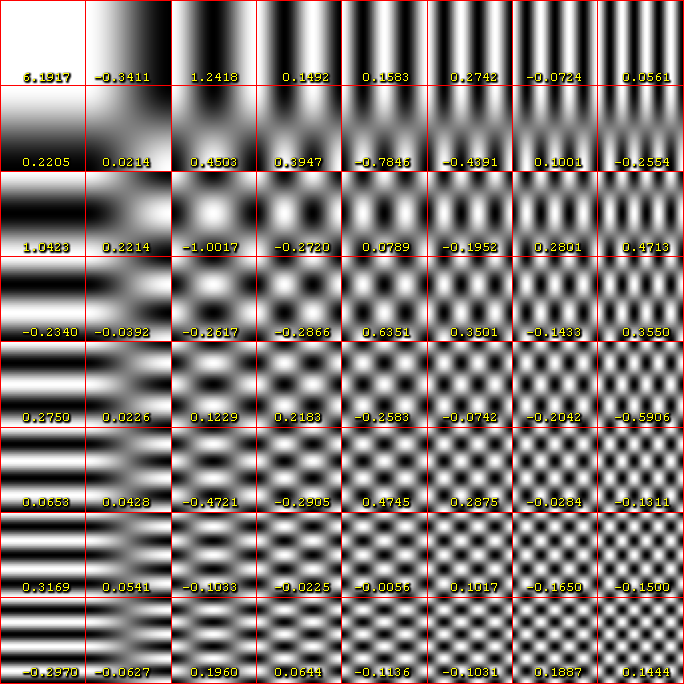
\includegraphics[width = .23\textwidth]{Dct-table.png}	
		}
		\hspace{0.3cm}
		\subfloat[原始图像(左)、右边四列置零(中)、左边四列置零(右)\label{fig2:fi2}]{
			
\includegraphics[width = .23\textwidth]{../source/3.2/origin.jpg}
			\hspace{0.05cm}					
			
\includegraphics[width = .23\textwidth]{../source/3.2/rightzero.jpg}
			\hspace{0.05cm}
			
\includegraphics[width = .23\textwidth]{../source/3.2/leftzero.jpg}
		}	
		\caption{题4.3~结果图}
		\label{fig2}
	\end{figure}
	从Figure~\ref{fig2:fi1} \citep{wiki2016}中可以看出dct系数右侧四列基底在横向上都有高频变化,而左边四列在横向上有低频变化。因此当右侧四列置零时,图像中的横向高频分量丢失,反之当左侧四列置零时,图像中横向低频分量丢失。
	
	测试结果如图Figure~\ref{fig2:fi2}所示。由于我所选择的图片在横向上没有高频变化,主要集中在低频变化上。因此右侧四列原本的值即较小,置零后对图片没有较大的影响,而左侧四列置零后,对图片的影响较大。如结果图所示,左侧四列置零后,整个图片都是黑蒙蒙的一片。
	
	具体代码如Listing~\ref{lst2:lst3}所示。
	
	\lstinputlisting[language=Matlab,caption=涂棋格代码,label=lst2:lst3,frame=shadowbox,
	backgroundcolor=\color{white}, rulesepcolor=\color{red!10!green!10!blue!10},,xleftmargin=2em,xrightmargin=2em, aboveskip=1em]{../source/3.2/M2_3.m}
	
		\subsection{若对DCT系数分别转置、旋转90度和旋转180度操作(rot90),逆变换后恢复的图像有何变化?}
		
		\begin{figure}[b]
			\centering
			\subfloat[原始图像\label{fig3:fi1}]{
				
\includegraphics[width = .2\textwidth]{../source/3.2/origin_rot.jpg}
			}
			\hspace{0.65cm}
			\subfloat[转置图像\label{fig3:fi2}]{
				
\includegraphics[width = .2\textwidth]{../source/3.2/transpose.jpg}
			}
			\hspace{0.65cm}
			\subfloat[旋转$90^\circ$ \label{fig3:fi3}]{
				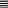
\includegraphics[width = .2\textwidth]{../source/3.2/rightrot90.jpg}
			}
			\hspace{0.65cm}
			\subfloat[旋转$180^\circ$ \label{fig3:fi4}]{
				
\includegraphics[width = .2\textwidth]{../source/3.2/rightrot180.jpg}
			}				
			\caption{题4.4~结果图}
			\label{fig3}
		\end{figure}
		若对DCT系数进行转置,则横纵分量的系数发生互换,因此恢复出来的原图像发生了转置。
		
		若对DCT系数逆时针旋转$90^\circ$,则大部分能量集中到左下角。而左下角系数代表的是横向低频变化、纵向高频变化,因此恢复出来的图像应当在横向上是低频变化,而纵向上呈现量化高频变化。
		
		若对DCT系数逆时针旋转$180^\circ$,则大部分能量集中到右下角。而右下角系数代表的横向纵向都是高频变化,因此恢复出来的在横纵向上都有量化高频变化。
		
		最终恢复出来的结果如图Figure~\ref{fig3}所示,与理论匹配。具体的代码如Listing~\ref{lst2:lst4}所示。
		
		\lstinputlisting[language=Matlab,caption=涂棋格代码,label=lst2:lst4,frame=shadowbox,
		backgroundcolor=\color{white}, rulesepcolor=\color{red!10!green!10!blue!10},,xleftmargin=2em,xrightmargin=2em, aboveskip=1em]{../source/3.2/M2_4.m}
		
		\subsection{如果认为差分编码是一个系统,请绘出这个系统的频率响应,说明他是怎样的滤波器。DC系统先进行差分编码在进行熵编码,说明他是一个怎样的系统。}
		
		不考虑初值,差分方程为:
		\begin{center}
			$ \hat{c}_{D}(n) = c_{D}(n-1) - c_{D}(n) $
		\end{center}
		
		\begin{figure}[H]
			\centering
			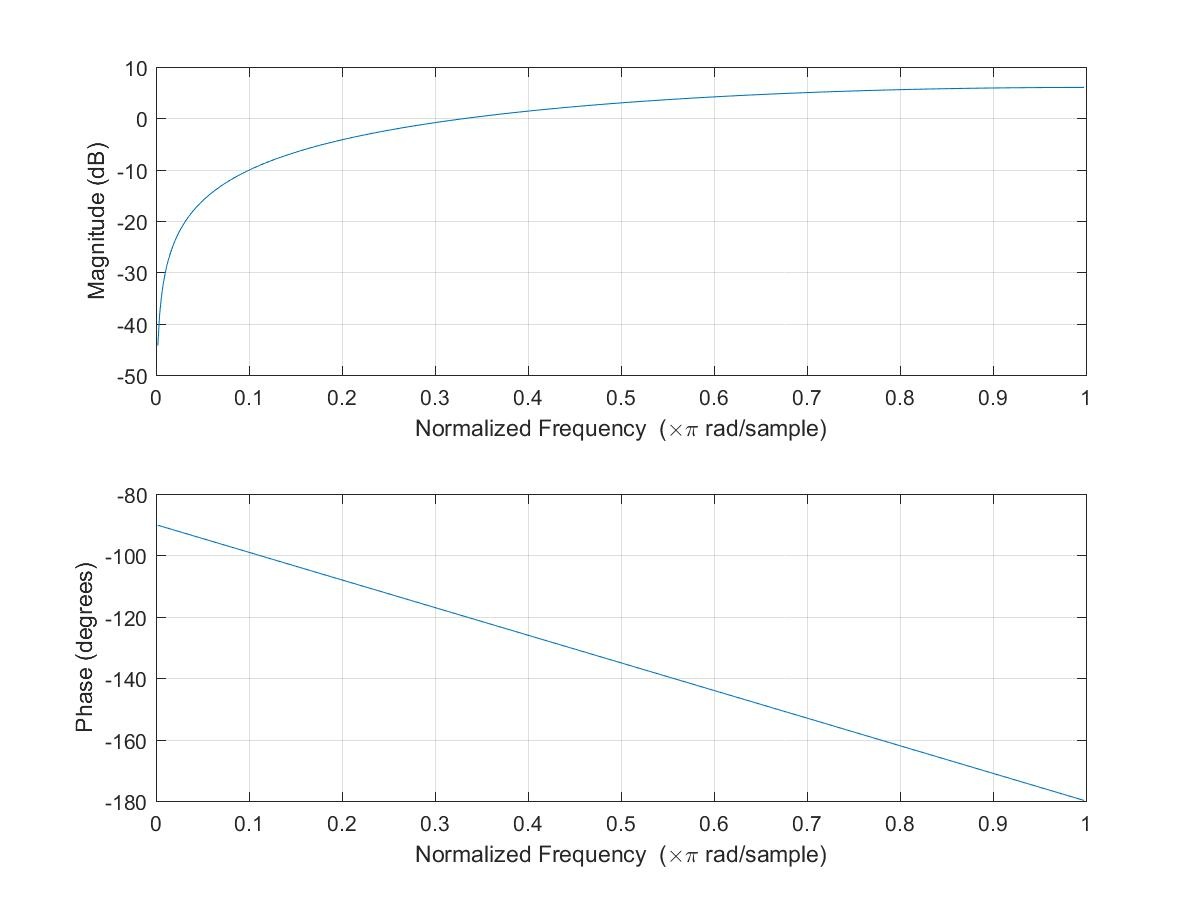
\includegraphics[width = .55\textwidth]{../source/3.2/frequency_plot.jpg}
			\caption{频率响应}
			\label{fig4}
		\end{figure}
		
		即$ A = [1], B = [-1\ 1] $,直接使用MATLAB的freqz函数即可画出频率响应,即Figure~\ref{fig4}。
		代码如Listing~\ref{lst2:lst5}所示。
		
		\lstinputlisting[language=Matlab,caption=频率响应代码,label=lst2:lst5,frame=shadowbox,
		backgroundcolor=\color{white}, rulesepcolor=\color{red!10!green!10!blue!10},,xleftmargin=2em,xrightmargin=2em, aboveskip=1em]{../source/3.2/M2_5.m}
		
		因此这是一个高通系统。而DC系统先进行差分编码再进行熵编码说明DC系统的低频分量较多,故经过系统后能量会有很大的衰减,从而实现信息压缩。
		
		\subsection{DC预测误差取值和Category值有何关系?如何利用预测误差计算出其Category?}
		
		从表中不难观察出,DC误差的取值所对应的二进制长度即为Category值。用数学表达式表述为:
		\begin{center}
			$ Category = ceil(log_2(|value| + 1)) $
		\end{center}
		
		\subsection{你知道哪些实现Zig-Zag扫描方法?请利用MATLAB强大功能设计一种最佳方法。}
		
		共有两种方法:
		
		第一种方法是知己将表格制作好,然后直接存在MATLAB中。这种方法需要自己实现编写好已知位数的zig-zag顺序列表,较为笨拙,但是实际程序运行时效率较高。本实验中采用的便是这种方法,但是效率较高。具体代码见Listing~\ref{lst2:lst6}。
		
		\lstinputlisting[language=Matlab,caption=zigzag代码,label=lst2:lst6,frame=shadowbox,
		backgroundcolor=\color{white}, rulesepcolor=\color{red!10!green!10!blue!10},,xleftmargin=2em,xrightmargin=2em, aboveskip=1em]{../source/3.2/zigzag.m}
		
		第二种方法是设置较为复杂的边界条件,每次碰到边界则横移转向/数移转向。这样的方法可以方便的生成任意尺寸的zig-zag序列,但是每次生成一次序列所需的时间较长,效率较低。因此我采用的是前一种zig-zag生产方法。
		
		\subsection{对测试图像分块、DCT和量化,将量化后的系数写成矩阵的形式,其中每一列为一个块的DCT系数Zig-Zag扫描后形成的列矢量,第一行为各个块儿的DC系数。}
		
		有了上述的Zig-Zag列后,可以很容易的将DCT系数按顺序变为一个列向量,然后放入矩阵中,代码清单Listing~\ref{lst2:lst11}中的代码可以实现这个目的。
		
		\lstinputlisting[language=Matlab,caption=coef矩阵代码,label=lst2:lst11,frame=shadowbox,
		backgroundcolor=\color{white}, rulesepcolor=\color{red!10!green!10!blue!10},,xleftmargin=2em,xrightmargin=2em, aboveskip=1em]{../source/3.2/M2_8.m}
		
		\subsection{请实现JPEG编码,输出为DC系数的码流、AC系数的码流、图像高度和图像宽度,将这四个变量写入jpegcodes.mat文件}
		
		为实现JPEG编码需要按照分块、DCT、量化、熵编码的顺序进行编码。
		
		\subsubsection{分块、DCT、量化}
		
		为了实现分块,需要原图像的宽和高的像素数目都为8的倍数。本大作业使用的hall\_gray的宽高都恰为8的倍数,若宽高不为高的倍数时,将其扩展到离他最近的8的倍数的宽高。新增的像素点用与其相邻的左侧的像素点或上侧的像素点填充。
		
		获得新的图像后,便可以进行$8 \times 8$的分块了与DCT变换了。修改图片像素尺寸的代码见Listing~\ref{lst2:lst7} 10-20行。
		
		\subsubsection{DC熵编码}
		
		DC系数即为coef矩阵的第一行。首先我们要对这一行系数做一个差分处理,从而消除低频分量达到压缩的目的。差分部分的代码见Listing~\ref{lst2:lst7} 30-36行。差分处理完成后将根据误差的值计算其对应的Category编号,见Listing~\ref{lst2:lst7} 第38行。而第40行对应的是根据Category编号查找Huffman编码,第41-51行对应的是将差分值的二进制编码与Huffman编码编入码流的过程。其中若差分值为负数,则将其1-补码编入码流中。
		
		\subsubsection{AC熵编码}
		
		DC系数处理完成后,我们继续处理AC熵编码。依次从矩阵中按列取出处理AC系数。	我的处理方法为找到这列系数中的非零值的位置,根据这些位置可以计算出他们前面分别有几个零。若是零的个数多余15个,则插入ZRL,并将计数器中的零的个数减十六,直到计数器中零的个数不大于15(Listing~\ref{lst2:lst7} 66-69行),
		在按照run/size查找Huffman码(Listing~\ref{lst2:lst7} 74行)。再对amp进行二进制编码便一并加入到码流中。查找方法与编码方法与DC编码一致,将所有非零值处理完成后,插入结束码(Listing~\ref{lst2:lst7} 79行)便可结束这一列的AC编码,加载下一列进行处理。
		
		
		\lstinputlisting[language=Matlab,caption=JPEG编码代码,label=lst2:lst7,frame=shadowbox,
		backgroundcolor=\color{white}, rulesepcolor=\color{red!10!green!10!blue!10},,xleftmargin=2em,xrightmargin=2em, aboveskip=1em]{../source/3.2/M2_9.m}
		
		\subsection{计算压缩比}
		
		计算压缩比时,需要注意将hall\_gray矩阵数据的uint8格式转为二进制长度,即8位之后在进行压缩比的比较。计算代码与结果见Listing~\ref{lst2:lst8}。
		\lstinputlisting[language=Matlab,caption=计算压缩比代码,label=lst2:lst8,frame=shadowbox,
		backgroundcolor=\color{white}, rulesepcolor=\color{red!10!green!10!blue!10},,xleftmargin=2em,xrightmargin=2em, aboveskip=1em]{../source/3.2/M2_10.m}
		
		\subsection{请实现JPEG解码,输入是你生成的jpegcodes.mat文件。分别用客观(PSNR)和主观方法评价编解码效果如何。}
		
		为了实现JPEG解码,我们需要定位每一个Huffman码的位置。由于不论是AC编码的Huffman编码还是DC编码的Huffman编码,每个Huffman编码都不是其他码的前缀码,因此可以维护一个目录,逐位比较,若是不相同,则将其从目录中删去,直至目录中只剩下一个条目为止。确定了条目后,便可得到所应该读去的amp的字长,或者是否需要去掉16个零。将amp读取并从2进制转为10进制后,便完成了解码的过程。接下来对DC差分系数则做一次反差分,获得原来的系数,对AC系数将解码得到的系数按照zigzag的顺序恢复到原来的$ 8 \times 8 $的矩阵中。取得原来的经过量化后的矩阵后,用 .* 来反量化得到原系数,再用idct2函数进行反dct变换,加上128后得到原始图像。从而实现JPEG的解码。具体的解码过程代码参见Listing~\ref{lst2:lst9}。
		
		\lstinputlisting[language=Matlab,caption=JPEG解码代码,label=lst2:lst9,frame=shadowbox,
		backgroundcolor=\color{white}, rulesepcolor=\color{red!10!green!10!blue!10},,xleftmargin=2em,xrightmargin=2em, aboveskip=1em]{../source/3.2/M2_11.m}
		
		而对于结果而言,JPEG编码前的图片如Figure~\ref{fig5:fi1}所示,而JPEG编解码后恢复的图片如Figure~\ref{fig5:fi2}所示。从主观的角度上看,大礼堂和两侧的树的细节都被编码压缩变得模糊,JPEG编码还是使得图片的细节有较大的损失。而从客观上来看PSNR的值为31.1874,有着较高的相似度。信息损失较小。
		
		\begin{figure}[h]
			\centering
			\subfloat[原始图像\label{fig5:fi1}]{
				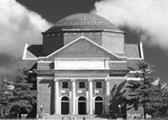
\includegraphics[width = .26\textwidth]{../source/3.2/hall_gray.jpg}
			}
			\hspace{0.75cm}
			\subfloat[解码图像\label{fig5:fi2}]{
				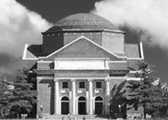
\includegraphics[width = .26\textwidth]{../source/3.2/decode.jpg}
			}				
			\caption{题4.11~结果图}
			\label{fig5}
		\end{figure}
		
		\subsection{将量化步长减小为原来一半,重做编解码。同标准量化步长的情况比较压缩比和图像质量。}
		
		即将使用的量化步长矩阵QTAB变为QTAB/2,再进行编解码。代码如Listing~\ref{lst2:lst10},结果对比图如Figure~\ref{fig6}所示。图片压缩比为ratio = 4.4097, 因此减半量化步长,会降低压缩比。图片质量上,从主观上看,细节比上一问要丰富了一些,但是比起原图仍然有损失;从客观上看,PSNR值为34.1754,图片的质量提高了。
		
		综上,减半量化步长会以牺牲压缩比的方式提高图片质量。
		
		\begin{figure}[t]
			\centering
			\subfloat[原始图像\label{fig6:fi1}]{
				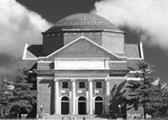
\includegraphics[width = .26\textwidth]{../source/3.2/hall_gray.jpg}
			}
			\hspace{0.75cm}
			\subfloat[半量化步长解码图像\label{fig6:fi2}]{
				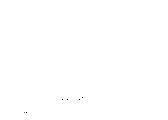
\includegraphics[width = .26\textwidth]{../source/3.2/halfqulidecode.jpg}
			}				
			\caption{题4.12~结果图}
			\label{fig6}
		\end{figure}
		
		\lstinputlisting[language=Matlab,caption=半量化步长代码,label=lst2:lst10,frame=shadowbox,
		backgroundcolor=\color{white}, rulesepcolor=\color{red!10!green!10!blue!10},,xleftmargin=2em,xrightmargin=2em, aboveskip=1em]{../source/3.2/M2_12.m}
		
		\subsection{看电视时偶尔能看到美丽的雪花图像(见snow.mat),请对其编解码。和测试图像的压缩比和图像质量进行比较,并解释比较结果。}
		代码与前述基本相同因此不在此处赘述。所得结果对比图如Figure~\ref{fig7}。
		
		雪花图像的压缩比为 3.6450,大幅下降。同样大幅下降的还有PSNR,为22.9244。观察图片来看,解码后有的地方被抹平了。
		
		原因解释起来,是因为标准量化步长中的高频的步长较大,因此高频损失较大。若是像是雪花图像这样各个交流分量比较平均的图片经过JPEG编码之后,会有较大的损失。不过雪花画面由于原本就比较混乱,因此损失了之后视觉上也没有较大的影响。
		
		\begin{figure}[b]
			\centering
			\subfloat[原始图像\label{fig7:fi1}]{
				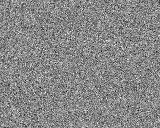
\includegraphics[width = .3\textwidth]{../source/3.2/snow.jpg}
			}
			\hspace{0.75cm}
			\subfloat[解码图像\label{fig7:fi2}]{
				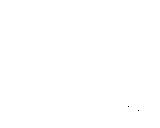
\includegraphics[width = .3\textwidth]{../source/3.2/decodesnow.jpg}
			}				
			\caption{题4.13~结果图}
			\label{fig7}
		\end{figure}
		
		\section{信息隐藏}
		
		\subsection{实现本章介绍的空域隐藏方法和提取方法。验证其抗JPEG编码能力。}
		
		\begin{figure}[t]
			\centering
			\subfloat[原始图像\label{fig17:fi1}]{
				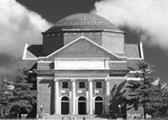
\includegraphics[width = .3\textwidth]{../source/3.3/hallgray.jpg}
			}
			\hspace{0.75cm}
			\subfloat[空域隐藏后图像\label{fig17:fi2}]{
					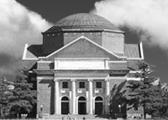
\includegraphics[width = .3\textwidth]{../source/3.3/Afterhidden.jpg}
			}
			\caption{题5.1~结果图}
			\label{fig17}
		\end{figure}
		
		为了方便提取,我们在隐藏的信息比特流之前加入表示长度的32位比特流。使用bitget函数可以方便的得到长度的32位比特流。而隐藏信息的时候,使用bitset将亮度值在uint8的格式下,将最小端的那一位设置为信息位的值,从而将信息隐藏进去。因此相当于每8个亮度值能隐藏一个字符。隐藏信息的算法见Listing~\ref{lst3:lst1}~1-56行。隐藏后的图像可以见结果对比图Figure~\ref{fig17}。
		
		而在解码上,首先先解出隐藏的标识信息流长的32位比特流,然后按照长度去解出信息。但是由于JPEG编码有压缩损失,导致我们最终得到的解码会有较大的错误,隐藏的信息几乎不可能解出来。因此尽管图片主观看不出来空域隐藏了信息,但是对于JPEG编码而言是一个较为无效的隐藏方法。
		
		\lstinputlisting[language=Matlab,caption=空域隐藏代码,label=lst3:lst1,frame=shadowbox,
		backgroundcolor=\color{white}, rulesepcolor=\color{red!10!green!10!blue!10},,xleftmargin=2em,xrightmargin=2em, aboveskip=1em]{../source/3.3/M3_1.m}
		
		\subsection{依次实现本章介绍的三种变换域信息隐藏方法和提取方法,分析嵌密方法的隐蔽性以及嵌密后JPEG图像的质量变化和压缩比变化}
			
		无论是采用哪一种方法隐藏信息,都是在DCT量化之后,因此提取信息应当在反量化以前。下列三种方法都是基于前一问的JPEG的编解码方法。在量化后加入隐藏信息编码的代码与在反量化前加入提取信息的代码。
		
		\begin{figure}[t]
			\centering
			\subfloat[5.2-1~结果图\label{fig10:fi1}]{
				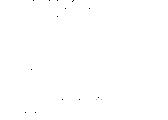
\includegraphics[width = .3\textwidth]{../source/3.3/firsthidden.jpg}
			}
			\hspace{0.2cm}
			\subfloat[5.2-2~结果图\label{fig10:fi2}]{
				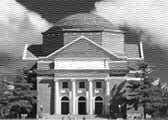
\includegraphics[width = .3\textwidth]{../source/3.3/secondhidden.jpg}
			}
			\hspace{0.2cm}
			\subfloat[5.2-3~结果图\label{fig10:fi3}]{
				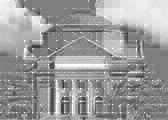
\includegraphics[width = .3\textwidth]{../source/3.3/thirdhidden.jpg}		
			}
			\caption{题5.2~结果图}
			\label{fig10}
		\end{figure}
		
		第一种方法:
		
		将每个量化后的dct系数最低位用信息位替代。该步骤在量化后,zigzag之前。在插入具体隐藏信息前,仍然插入表示信息长度的32位信息流后,再插入具体的隐藏的信息。由于每个dct系数的最低位都被当成信息位,因此本方法可以隐藏较多的信息。
		
		对于解码部分,则是先解出前32位得到隐藏的信息长度,在根据得到的长度决定什么时候停止获取隐藏的信息位,然后在翻译回信息。
		
		而这种所得的结果图如Figure~\ref{fig10:fi1}。由结果可以看出来,这种方式换对画面产生非常明显的影响,因为每一位dct系数都被修改,特别是原来较小的的dct系数被修改,所以原来的$ 8 \times 8$的方块在idct后变得不那么连续了,复原的图像隐藏过信息就比较明显。具体代码见Listing~\ref{lst3:lst2} 。
		
		\lstinputlisting[language=Matlab,caption=第一种变化域代码,label=lst3:lst2,frame=shadowbox,
		backgroundcolor=\color{white}, rulesepcolor=\color{red!10!green!10!blue!10},,xleftmargin=2em,xrightmargin=2em, aboveskip=1em]{M3_2_1.m}
		
		第二种方法:
		
		第二种方法与第一种方法大体相似,唯一的区别在于仅仅选择部分dct系数进行信息隐藏。这里我在64个dct系数中选择前16个系数进行信息隐藏。之后解码时,也仅对前16个系数进行信息位的读取,获得隐藏的信息。本方法部分关键代码与上一种非常相似,因此不在此处列出。结果对比图如Figure~\ref{fig10:fi2}所示。由于前16个系数在横向上低频敏感在纵向上影响葱低频到高频。因此最终得到的图像可以看到在纵向上有明显的量化感与修改感。这种隐藏方式,比第一种要隐蔽一些,但是其能够隐藏的信息量比第一种方法要少。而且其图片修改感仍然非常明显。
		
		第三种方法:
		
		第三种方法与前两种不同。第三种方法在zig-zag序列化之后进行信息隐藏,且每64个系数只能隐藏1个信息位。因此这种方法能隐藏的信息量非常有限。这个方式的编解码都比较简单。编码只需要找到最后一个非零的数,替换其后的一个零为信息位;若是最后一个非零的数是最后的数,则直接替换其为信息位。解码则直接找到最后一位非零的数,提取出来作为信息位即可。
		
		这种隐藏方式的关键代码如Listing~\ref{lst3:lst4}所示。结果对比图如Figure~\ref{fig10:fi3}所示。可以发现这种方式,对图片几乎没有影响,但是其能够隐藏的信息量实在太少了!
		
		\lstinputlisting[language=Matlab,caption=第三种变化域代码,label=lst3:lst4,frame=shadowbox,
		backgroundcolor=\color{white}, rulesepcolor=\color{red!10!green!10!blue!10},,xleftmargin=2em,xrightmargin=2em, aboveskip=1em]{./M3_2_3.m}
		
		\subsection{请设计实现新的隐藏算法并分析其优缺点}
		
		\begin{figure}[h]
			\centering
			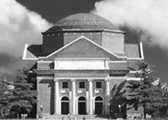
\includegraphics[width = .3\textwidth]{../source/3.3/myselfhidden.jpg}		
			\caption{题5.3~结果图}
			\label{fig11}
		\end{figure}
		
		如前述三种方法的结果所示,前两种方法可以隐藏大量信息,但是对原图片的影响较大;第三种方法对原图片几乎没有影响,但是能够隐藏的信息量过小。因此希望能够设计一种折中的方法来进行信息的隐藏。
		
		这里设计了一种方法。当被修改的系数足够大的时候,信息位被修改对原图片的影响便不会很大。因此在此设定了负数上界与正数下界,凡是不小于正数下界或不大于负数上界的数,都可以被允许修改信息位。这里设定的正数下界为6,负数上界为-正数下界+1。设定正数下界为偶数的原因是希望信息位被修改后,能能符合边界条件,在解码的时候能够被正确的被读出。负数上界为奇数的原理相同。
		
		本方法进行信息隐藏时的过程发生在zig-zag序列化后,解读信息发生在zig-zag复原前。同理,本方法在隐藏信息前仍然放入了8位的标识长度的长度码。
		
		本方法关键代码如Listing~\ref{lst3:lst5}
		\lstinputlisting[language=Matlab,caption=自行设计方法代码,label=lst3:lst5,frame=shadowbox,
		backgroundcolor=\color{white}, rulesepcolor=\color{red!10!green!10!blue!10},,xleftmargin=2em,xrightmargin=2em, aboveskip=1em]{./M3_3.m}
		
		\section{人脸识别}
		
		\subsection{所给资料Faces目录下包含从网络中截取的28张人脸,试以其作为样本训练人脸标准v}
		\subsubsection{样本人脸大小不一致,是否需要首先将图像调整为相同大小}
		
		不需要。因为图片的大小对各个颜色出现的频率比例没有影响。
		
		\subsubsection{假设L = 3,4,5,所得的三个v之间有什么关系?}
		
		为了方便后续函数调用,共编写了图片量化函数quantized\_pic(Listing~\ref{lst4:lst1})和特征获取函数get\_feature(Listing~\ref{lst4:lst2})。量化函数将图片的$ 8 \times 3 $位颜色重新量化为 $ 8 \times L $种颜色。而特征获取函数获得颜色的频率特征向量。
		
		根据理论分析,人脸的颜色应当集中在一个区域内,因此,最后得到的v应该得当最多有$ 2^L$个大峰,每个大峰包含最多$ 2^L $个小峰。因此L每增大一位大峰和小凤的数量增加一倍,这也是量化越来越细化的体现。最终结果图见Figure~\ref{fig12}。
		
		\begin{figure}[h]
			\centering
			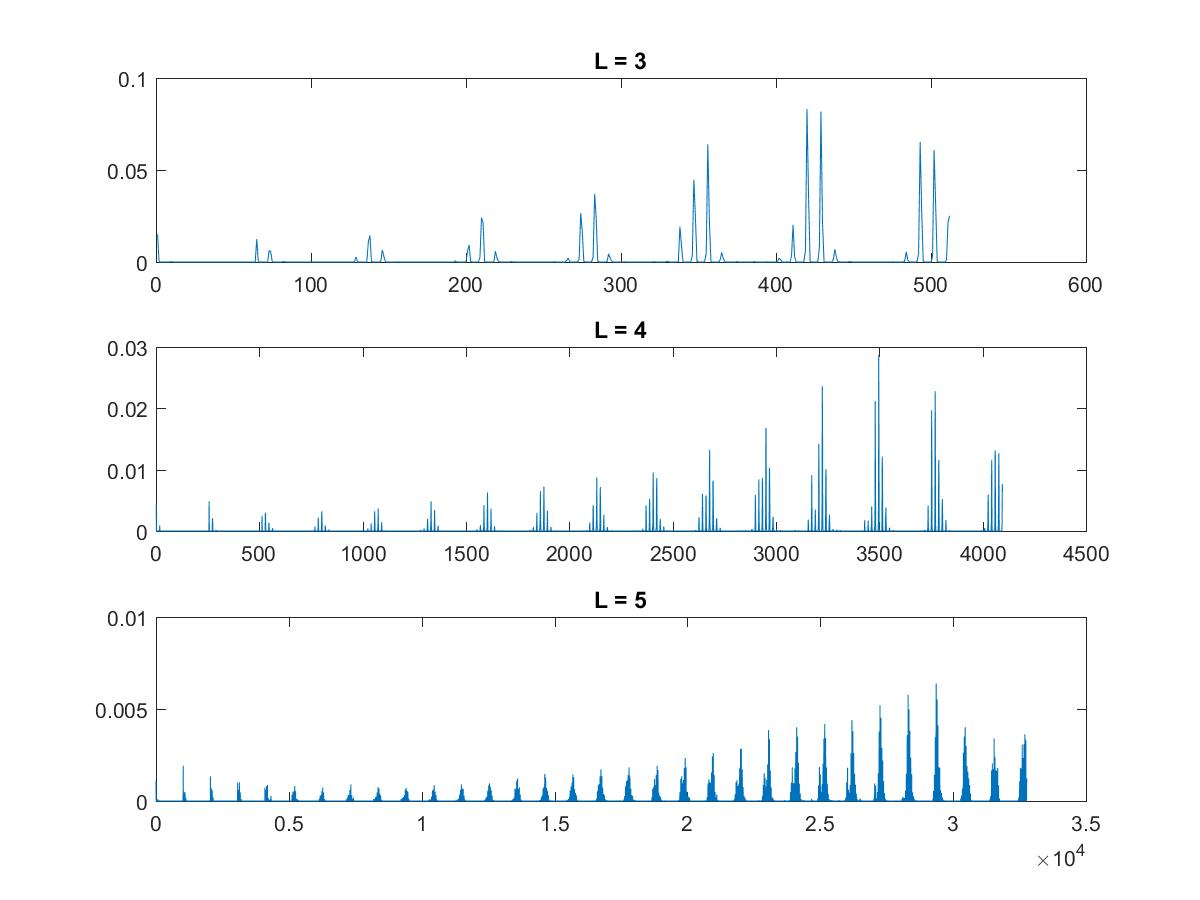
\includegraphics[width = .6\textwidth]{../source/3.4/L_from_three_to_five.jpg}
			\caption{题6.2~结果图}
			\label{fig12}
		\end{figure}
	
		\lstinputlisting[language=Matlab,caption=量化图片代码,label=lst4:lst1,frame=shadowbox,
		backgroundcolor=\color{white}, rulesepcolor=\color{red!10!green!10!blue!10},,xleftmargin=2em,xrightmargin=2em, aboveskip=1em]{../source/3.4/quantized_pic.m}
		
		\lstinputlisting[language=Matlab,caption=获得频率特征代码,label=lst4:lst2,frame=shadowbox,
		backgroundcolor=\color{white}, rulesepcolor=\color{red!10!green!10!blue!10},,xleftmargin=2em,xrightmargin=2em, aboveskip=1em]{../source/3.4/get_feature.m}
		
		\lstinputlisting[language=Matlab,caption=运行代码,label=lst4:lst3,frame=shadowbox,
		backgroundcolor=\color{white}, rulesepcolor=\color{red!10!green!10!blue!10},,xleftmargin=2em,xrightmargin=2em, aboveskip=1em]{../source/3.4/M4_1.m}
		
		\subsection{设计一种从任意大小的图片中检测任意多张人脸的算法并编程实现(输出图像在判定为人脸的位置加上红色的方框)。随意选取一张多人的照片,对程序进行测试。尝试L分别取不同的值,评价检测结果的区别。}
		
		\begin{figure}[h]
			\centering
			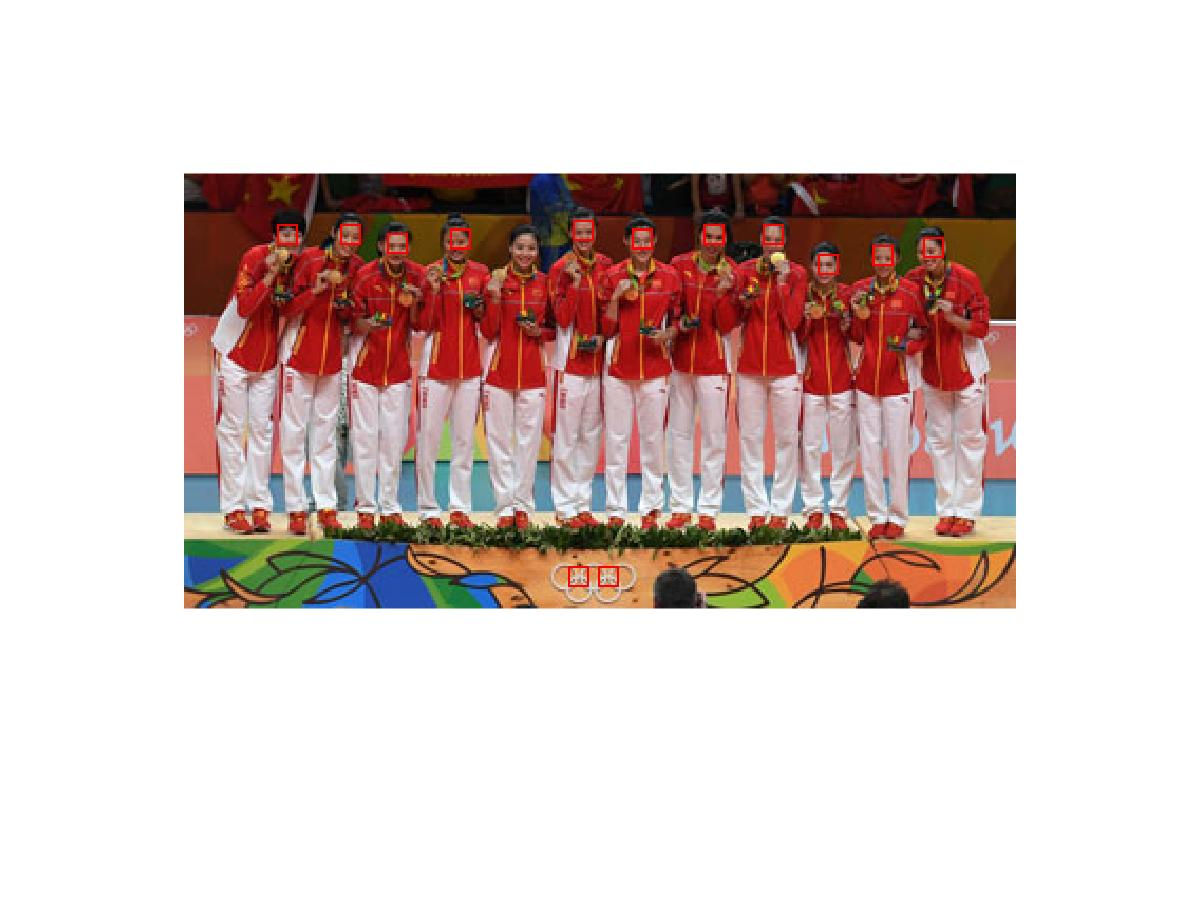
\includegraphics[width = .8\textwidth]{../source/3.4/face_recongnize.jpg}	
			\caption{题6.3~结果图}
			\label{fig13}
		\end{figure}
		
		首先需要对整个图片进行分块取样。然后对每个取样图块计算其与训练样本的距离,距离小于一定阈值的加入到候选人脸队列中。之后遍历候选人脸队列,按照距离从小到大排列,依次将不相互覆盖的图块加入人脸序列完成最后的识别。我们选择2016年里约奥运会女排的颁奖图片进行测试,最终的结果如图Figure~\ref{fig13}所示。可以看出大多数人脸都被识别出来,只有一位脸较黑的队员的脸没有被识别出来。不过奥运五环的地方的频率比和人脸较为相似,也被识别为人脸。具体的识别算法见Listing~\ref{lst4:lst4}。

		\lstinputlisting[language=Matlab,caption=运行代码,label=lst4:lst4,frame=shadowbox,
		backgroundcolor=\color{white}, rulesepcolor=\color{red!10!green!10!blue!10},,xleftmargin=2em,xrightmargin=2em, aboveskip=1em]{../source/3.4/M4_2.m}
		
		\subsection{对上述图像分别进行如下处理后}
		
		\begin{figure}[h]
			\centering
			\subfloat[6.4-1~结果图\label{fig14:fi1}]{
				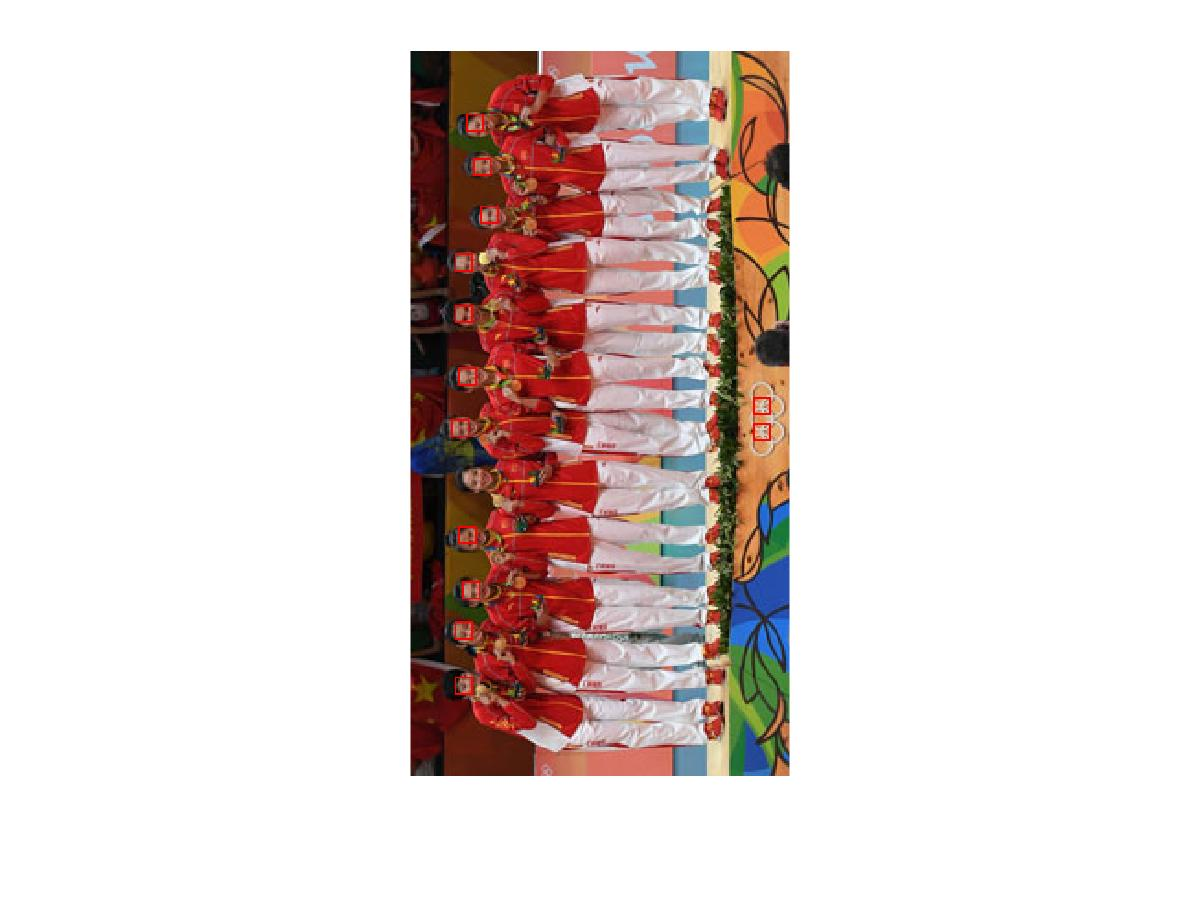
\includegraphics[width = .3\textwidth]{../source/3.4/rotation.jpg}
			}
			\hspace{0.2cm}
			\subfloat[6.4-2~结果图\label{fig14:fi2}]{
				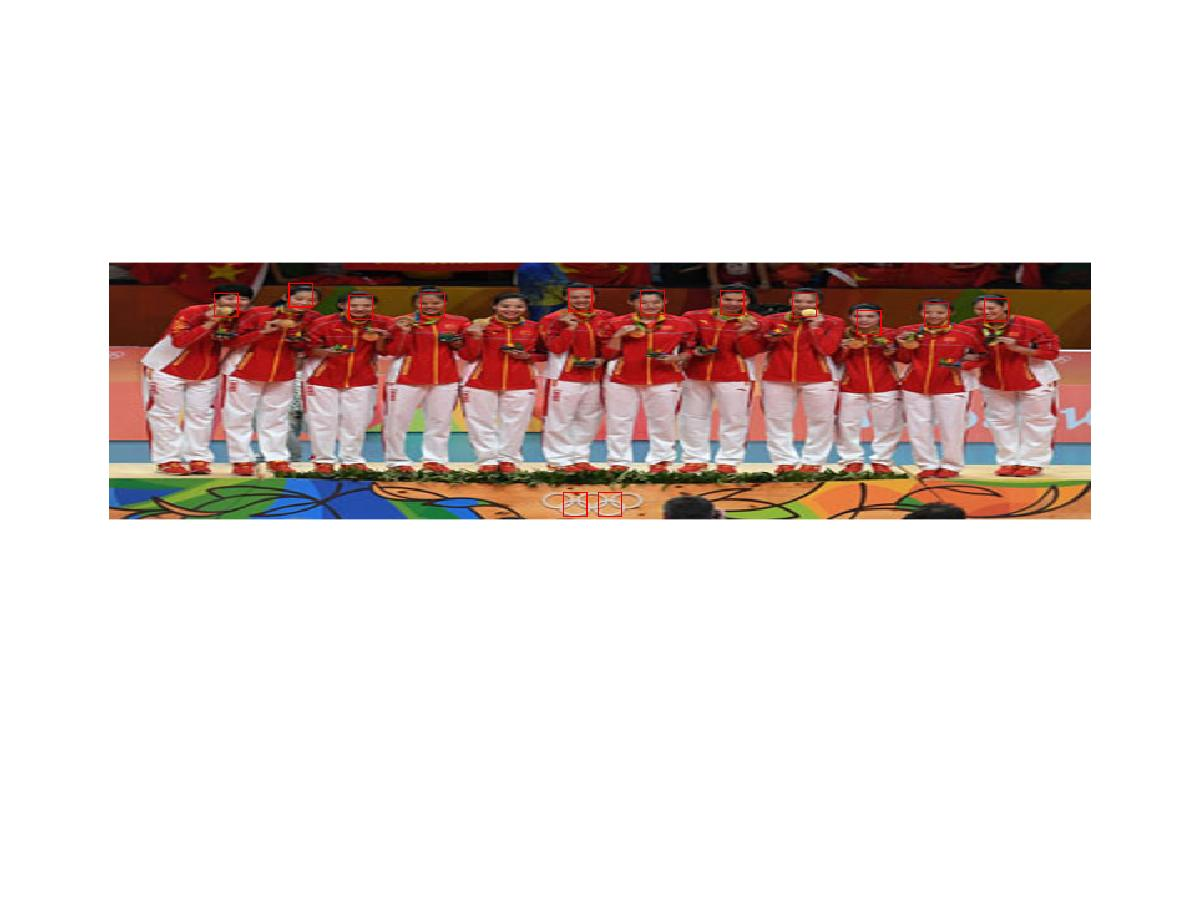
\includegraphics[width = .3\textwidth]{../source/3.4/resize.jpg}
			}
			\hspace{0.2cm}
			\subfloat[6.4-3~结果图\label{fig14:fi3}]{
				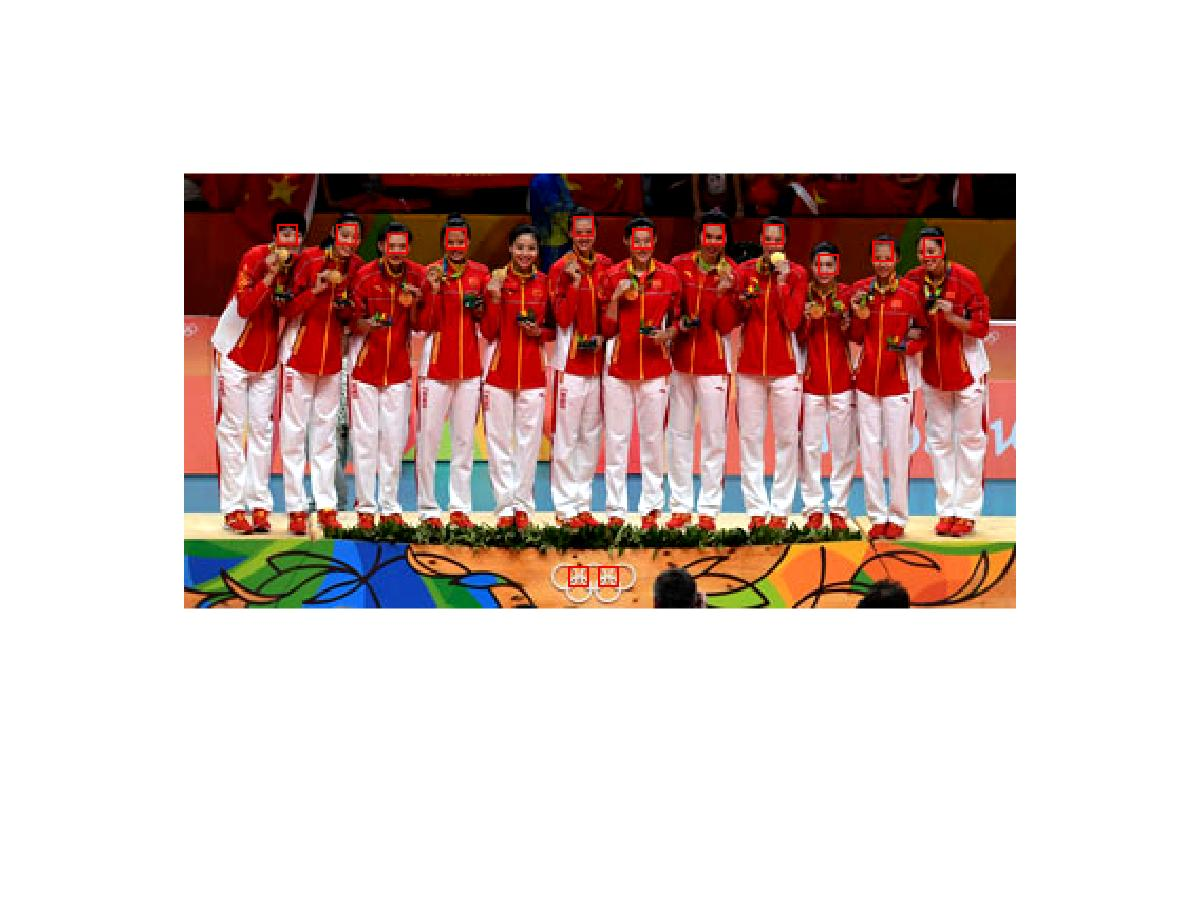
\includegraphics[width = .3\textwidth]{../source/3.4/imadjust.jpg}		
			}
			\caption{题6.4~结果图}
			\label{fig14}
		\end{figure}
		
		\subsubsection{顺时针旋转90度}
		
		旋转$ 90^\circ $后的识别结果如Figure~\ref{fig14:fi1}所示。
		
		\subsubsection{保持高度不变,宽度变为原来的2倍}
		
		保持高度不变,宽度变为原来2倍的识别结果如Figure~\ref{fig14:fi2}所示。
		
		\subsubsection{适当改变颜色}
		
		适当改变颜色后的识别结果如Figure~\ref{fig14:fi3}所示。
		
		通过上述结果显示,这种颜色频率特征的识别方法确实在一定程度上能够抗旋转、抗拉伸、与适当的颜色改变。但是若是碰到颜色较为相似的其他图片,则也会被误识别成为人脸而显示。
		
		
		\subsection{如果可以重新选择人脸样本的训练标准,你觉得应该如何选取?}
		
		首先选择的人脸应该要覆盖两个性别的不同年龄段的人,样本数量要足够多。其次,选取的人脸样本应该覆盖不同的皮肤种类。最后,建议不同的人种的脸分开训练,分别识别。这样才能较高的提高识别准确度,否则加入平均只会降低识别率。
		
		\section{实验总结}
		
		通过本次实验,我对图像的各种处理方式,对图片的压缩编码、图片识别、信息隐藏等方式都有了较为全面的认识!非常感谢谷哥哥为我们提供这样一个大作业,了解图片这种二维乃至多维信号等处理方式。通过本次实验,我收获颇丰!
		
		\renewcommand{\UrlFont}{\small\tt}
		\bibliographystyle{plain}
		\bibliography{document}
		
		\appendix
		\section{代码清单} \label{app:app1}
		
		根目录:/source
		\begin{enumerate}
			\item /3.1/a.m
			\item /3.1/b.m
			\item /3.2/M2\_1.m
			\item /3.2/M2\_2.m
			\item /3.2/M2\_3.m
			\item /3.2/M2\_4.m
			\item /3.2/M2\_5.m
			\item /3.2/M2\_7.m
			\item /3.2/M2\_8.m
			\item /3.2/M2\_9.m
			\item /3.2/M2\_10.m
			\item /3.2/M2\_11.m
			\item /3.2/M2\_12.m
			\item /3.2/M2\_13.m
			\item /3.2/zigzag.m
			\item /3.3/M3\_1.m
			\item /3.3/M3\_2\_1.m
			\item /3.3/M3\_2\_2.m
			\item /3.3/M3\_2\_3.m
			\item /3.3/M3\_3.m
			\item /3.3/Jepg.m
			\item /3.3/DeJepg.m
			\item /3.3/zigzag.m
			\item /3.4/M4\_1.m
			\item /3.4/M4\_2.m
			\item /3.4/M4\_3\_1.m
			\item /3.4/M4\_3\_2.m
			\item /3.4/M4\_3\_3.m
			\item /3.4/mydistance.m
			\item /3.4/get\_feature.m
			\item /3.4/quantized\_pic.m
		\end{enumerate}
		
\end{document}